\section{Trifocal Tensor}
\subsection{Tensor Notation}
Tensors are geometric objects used to represent linear relations between vectors, scalars, and other tensors. A tensor can be represented as a multi-dimensional array of numerical values. The order of a tensor is the dimensionality of the array needed to represent it. Scalars are single numbers and are thus 0th-order tensors. Vectors are 1-dimensional array, 1st-order tensors arranged in a column or row. Matrices are 2-dimensional arrays, 2nd-order tensors arranged as a 2D array of numbers. Similarly, a tensor with three indices may be thought as a 3D array of numbers.

Tensors provide a natural and concise mathematical framework for formulating and solving problems in areas of physics. Tensors express the relationship between vectors, hence they are independent of a particular choice of coordinate system.

The notation for a tensor is similar to that of a matrix, except that a tensor may have an arbitrary number of indices \textit{e.g.:}$A_{ijk\dotsb}$. In addition, a tensor with rank $r+s$ may be of mixed type $(r,s)$, consisting of $r$ \texttt{contravariant (upper)} indices and $s$ \texttt{covariant (lower)} indices. In tensor notation, a vector $v$ would be written $v_i$, where $i =1,\dotsb,m$, and a matrix is a tensor of type $(1,1)$ would be written as $A^{j}_{i}$.

Tensor notation can provide a very concise way of writing vector and more general identities. For example, the dot product $u.v$ can be simply written as
$$
u.v = u_{i}v^{i}
$$
where repeated indices are summed over. This is called \texttt{Einstein Summation}. It is a notational convention for simplifying expressions including summations of vectors, matrices and general tensors. The convention can be best illustrated through the following equation
$$
  c^{i}_{k} = a^{i}_{j}b^{j}_{k} = \sum_{j} a_{ij}b_{jk}
$$

Similarly, the cross product can be concisely written as
$$
  (u\times v)_{i} = \epsilon_{ijk} u^{j} v^{k},
$$
where $\epsilon_{ijk}$ is the permutation tensor defined for $r,s,t =1,\dotsb,3$ as follows:
$$
\epsilon_{rst} = \begin{cases}
  0 & \text{ unless } r,s \text{ and } t \text{ are distinct}\\
  +1 & \text{ if } rst \text{ is an even permutation of } 123\\
  -1 & \text{ if } rst \text{ is an odd permutation of } 123
\end{cases}
$$

\subsection{Three-View Geometry}
The Trifocal Tensor is a $3 \times 3 \times 3$ array of numbers that incorporates all projective geometric relationships among three views. It relates the coordinates of corresponding points or lines in three views, being independent of the scene structure and depending only on the relative motion among the three views and their intrinsic calibration parameters. Hence, the trifocal tensor can be considered as the generalization of the fundamental matrix in three views. It can also be seen as a collection of three rank-two $3 \times 3$ matrices $T_1, T_2, T_3$.

The geometric basis for the trifocal tensor can be deduced from the incidence relationship of three corresponding lines. We start by supposing a line 3-space is imaged in three views as in Figure.\ref{fig:threeviews}. The planes back-projected from the lines in each view must all meet in a single line in space, the 3D line that projects to the mated line in the three images. Since in general three arbitrary planes in space do not meet in a single line, this geometric incidence condition provides a genuine constraint on sets of corresponding lines.

\begin{figure}[ht!]
  \centering
  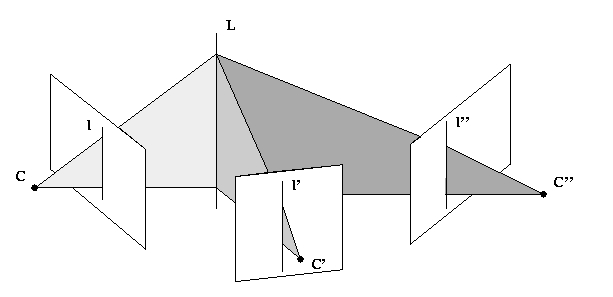
\includegraphics[width=100mm]{figures/threeviews.jpg}
  \caption{Trifocal geometry of three views}
  \label{fig:threeviews}
\end{figure}

Let $ l_i \leftrightarrow l^{\prime}_i \leftrightarrow l^{\prime \prime}_i $ be the set of corresponding lines of $L$. Let the camera matrices for the three views be $P =  \begin{bmatrix} I \mid 0 \end{bmatrix}$, $P^{\prime} = \begin{bmatrix} A \mid a_{4} \end{bmatrix}$, $P^{\prime \prime} = \begin{bmatrix} B \mid b_{4} \end{bmatrix}$, where $A$ and $B$ are $3 \times 3$ matrices, and the vectors $a_i$ and $b_i$ are the \texttt{i}-th columns of the respective camera matrices for $i = 1,\dotsb,4$. $A$ and $B$ are the homographies from the first to the second and third cameras respectively. Due to our choice for the first camera matrix, $a_4$ and $b_4$ are consequently the epipoles of the first camera in views two and three respectively.
 \begin{align*}
  a_4 &= e^{\prime} = P^{\prime}C  & b_4 &= e^{\prime \prime}  = P^{\prime \prime}C
 \end{align*}

Each image line back-projects to a plane as shown in Figure.\ref{fig:threeviews}. These planes are
\begin{align*}
\pi &= P^{T}l = \begin{pmatrix} l \\ 0 \end{pmatrix}  & \pi^{\prime} &= P^{\prime T}l^{\prime} = \begin{pmatrix} A^{T}l^{\prime} \\ a^{T}_{4}l^{\prime} \end{pmatrix} & \pi^{\prime \prime} &= P^{\prime \prime T}l^{\prime \prime} = \begin{pmatrix} B^{T}l^{\prime \prime} \\ b^{T}_{4}l^{\prime \prime} \end{pmatrix}
\end{align*}

The intersection constraint of the three planes in the common line in 3-space can be expressed algebraically by the requirement that the $4 \times 3$ matrix $ M = \begin{bmatrix} \pi & \pi^{\prime} & \pi^{\prime \prime} \end{bmatrix}$ has rank $2$. Points on the line of intersection may be represented as $X = \alpha X_1 + \beta X_2$, with $X_1$ and $X_2$ linearly independent. Such points lie on all three planes and so $\pi^{T}X = \pi^{\prime T}X = \pi^{\prime \prime T}X = 0$. It follows that $M^{T}X = 0$. Consequently M has a 2-dimensional null-space since $M^{T}X_1 = 0$ and $M^{T}X_2 =0$.

Since the rank of $M$ is 2, there is a linear dependence between its columns $m_i$, such that.
\begin{gather*}
M = \begin{bmatrix} m_1, m_2,m_3 \end{bmatrix} = \begin{bmatrix} l & A^{T}l^{\prime} & B^{T}l^{\prime \prime} \\
  0 & a^{T}_{4}l^{\prime} & b^{T}_{4}l^{\prime \prime}
\end{bmatrix}\\
m_1 = \alpha m_2 + \beta m_3
\end{gather*}

From the 2nd row of $M$, $\alpha = k(b^{T}_4 l^{\prime \prime})$ and $\beta = -k(a^{T}_4 l^{\prime})$ for some scalar $k$. Applying this back to the 1st row get
\begin{gather*}
l = (b^{T}_4 l^{\prime \prime })A^{T}l^{\prime} - (a^{T}_4 l^{\prime})B^{T}l^{\prime \prime}\\
l = (l^{\prime \prime T} b_{4})A^{T}l^{\prime} - (l^{\prime T} a_{4})B^{T}l^{\prime \prime}
\end{gather*}

The \texttt{i}-th coordinate $l_i$ of $l$ may be written as
\begin{gather*}
  l_i = l^{\prime \prime T} (b_{4}a^{T}_{i}) l^{\prime} - l^{\prime T}(a_{4}b^{T}_{i}) l^{\prime \prime}\\
  l_i = l^{\prime T} (a_{i}b^{T}_{4}) l^{\prime \prime} - l^{\prime T}(a_{4}b^{T}_{i}) l^{\prime \prime}
\end{gather*}

This relationship can be expressed with the permutation tensor such as
\begin{gather}
  \mathcal{T}_{i} = a_{i}b^{T}_{4} - a_{4}b^{T}_{i} \label{eq:trifocalgeometry1}\\
  l_i = l^{\prime T} \mathcal{T}_{i} l^{\prime \prime} \label{eq:trifocalgeometry2}
\end{gather}

$\mathcal{T}$ is then the trifocal tensor relating the 3 views together. It has 27 elements. There are 26 independent rations apart from the common overall scaling factor of the tensor. However, the tensor has only 18 independent degrees of freedom. Each of 3 camera matrices has 11 degrees of freedom which makes $33$ in total. However, $15$ degrees of freedom must be subtracted to account for the projective world frame, thus leaving 18 degrees of freedom.

\begin{figure}[ht!]
  \centering
  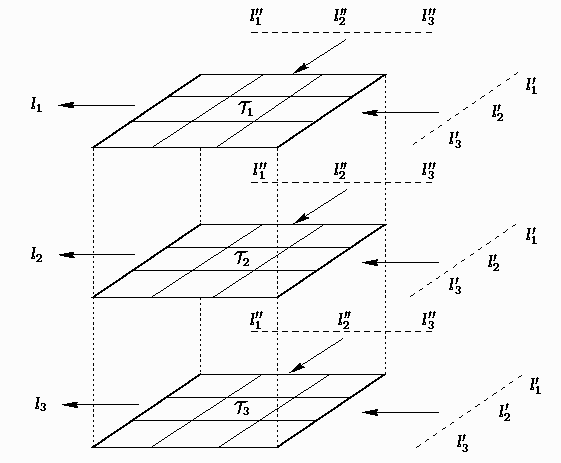
\includegraphics[width=100mm]{figures/trifocaltensor.png}
  \caption{\textbf{A 3D representation of the trifocal tensor}  $l_{i} = l_{j}^{\prime} l_{k}^{\prime \prime} \mathcal{T}_{i}^{jk}$ }
  \label{fig:trifocaltensor}
\end{figure}

A point $x$ on the line $l$ must satisfy $x^{T}l = \sum_{i} x^{i}l_{i} = 0$. From \eqref{eq:trifocalgeometry2}, this may be written as
$
l^{\prime T}(\sum_{i} x^{i}\mathcal{T}_{i}) l^{\prime \prime} = 0
$
which means that there exists a 3D point $X$ mapping to $x$ in the first image, and to points on the lines $l^{\prime}$ and $l^{\prime \prime}$ in the second and third images. It's the incidence relationship that holds point-line-line correspondence.

To develop the point-point-point correspondence relationship, we can explore the homography map between the points on first and third images given by $x^{\prime \prime} = Hx$ and $l = H^{T}l^{\prime \prime}$. Thus we get
$$
  h_i = \mathcal{T}^{T}_{i}l^{\prime}
$$
Similarly, the homography from the first to the second views
$$
  h_i = \mathcal{T}_{i}l^{\prime \prime}
$$

Using these results back to our point-line-line correspondence relation,
\begin{gather*}
  x^{\prime \prime} = (\sum_{i} x^{i}\mathcal{T}^{T}_{i}) l^{\prime}
  x^{\prime \prime T}[x^{\prime \prime}]_{\times} = l^{\prime T} (\sum_{i} x^{i}\mathcal{T}_{i})[x^{\prime \prime}]_{\times} = 0^{T}
\end{gather*}

The line $l^{\prime}$ passes through $x^{\prime}$ may be written as $l^{\prime} = [x^{\prime}]_{\times}y^{\prime}$ for some point $y^{\prime}$ on $l^{\prime}$. Then
$$
  y^{\prime T} [x^{\prime}]_{times} (\sum_{i} x^{i}\mathcal{T}_{i})[x^{\prime \prime}]_{\times} = 0^{T}
$$

This relation holds true for all lines $l^{\prime}$ through $x^{\prime}$ and so is independent of $y^{\prime}$, hence this relation can be written as
$$
[x^{\prime}]_{times} (\sum_{i} x^{i}\mathcal{T}_{i})[x^{\prime \prime}]_{\times} = 0_{3\times 3}
$$
which expresses the point-point-point coincidence relationship required. Expressing this relation in proper tensor notation is then given by
\begin{equation}
  x^{i}(x^{\prime j} \epsilon_{jpr})(x^{\prime \prime k} \epsilon_{kqs})\mathcal{T}^{pq}_{i} = 0_{rs} \label{eq:trifocalgeometry3}
\end{equation}

\subsection{Recovering Projection Matrices}
\label{sub:recovering_projection_matrices}
Since the trifocal tensor embeds the geometry of the three cameras in our scene, this implies that the camera matrices may be computed from the trifocal tensor up to a projective ambiguity~\cite{Hartley2004}.

First, the epipoles $e^{\prime},e^{\prime \prime}$ are retrieved. Let $u_i$ and $v_i$ be the left and right null-vectors respectively of $\mathcal{T}_{i}$, \textit{i.e.:} $u_{i}^{T} \mathcal{T}_{i} = {\bf 0}^{T}, \mathcal{T}_{i}v_i = 0$. Then the epipoles are obtained as the null vectors to the following $ 3 \times 3$ matrices:
\begin{equation}
  e^{\prime T} [u_1, u_2, u_3] = 0  \text{ and } e^{\prime \prime T}[v_1, v_2, v_3] = 0
\end{equation}

Next, to retrieve the camera matrices $P^{\prime}, P^{\prime \prime}$. The epipoles are normalized to unit norm, then:
\begin{equation}
  P^{\prime} = [[\mathcal{T}_{1}, \mathcal{T}_{2},\mathcal{T}_{3}] e^{\prime \prime} | e^{\prime}] \text{ and } P^{\prime \prime} = [(e^{\prime \prime} e^{\prime \prime T} - I)[\mathcal{T}_{1}^{T}, \mathcal{T}_{2}^{T},\mathcal{T}_{3}^{T}] e^{\prime} | e^{\prime \prime}]
\end{equation}


